\chapter{Introduction}
\label{cha:Introduction} % Ein Label ist optional, ermoeglicht aber die Referenzierung
\textbf{\color{green}THIS IS FINAL}

In this chapter we will explore the motivation and goals of this seminar thesis, as well its structure.
In order to do this, we will explain the motivation behind the topic as well as the research questions that we aim to answer in section \ref{sec:motivation-goals} \nameref{sec:motivation-goals}.
Afterwards we will then explain the thesis's structure and contents in section \ref{sec:structure} \nameref{sec:structure}.

\section{Motivation and Goals}
\label{sec:motivation-goals}
\textbf{\color{red}THIS IS NOT FINAL}

This chapter delves into the motivation behind this thesis and furthermore defines research questions, which we aim to answer in the subsequent chapters.

The advancements in technology of the past decades has lead to enormous data creation. Technology has become ubiquitous, 
with the evolution of cell phones to smartphones, the digitilization of industrial processes, Industry 4.0
and the increasing amount of ``smart`` devices, causing the creation of information to grow exponentially.
It is estimated that the \gls{datasphere} will reach the size of 175 zettabytes by 2025, as shown in figure \ref{fig:growth_datasphere}.
% Graph estimating the growth of the global datasphere (by IDC)
\begin{figure}[ht]
\centering
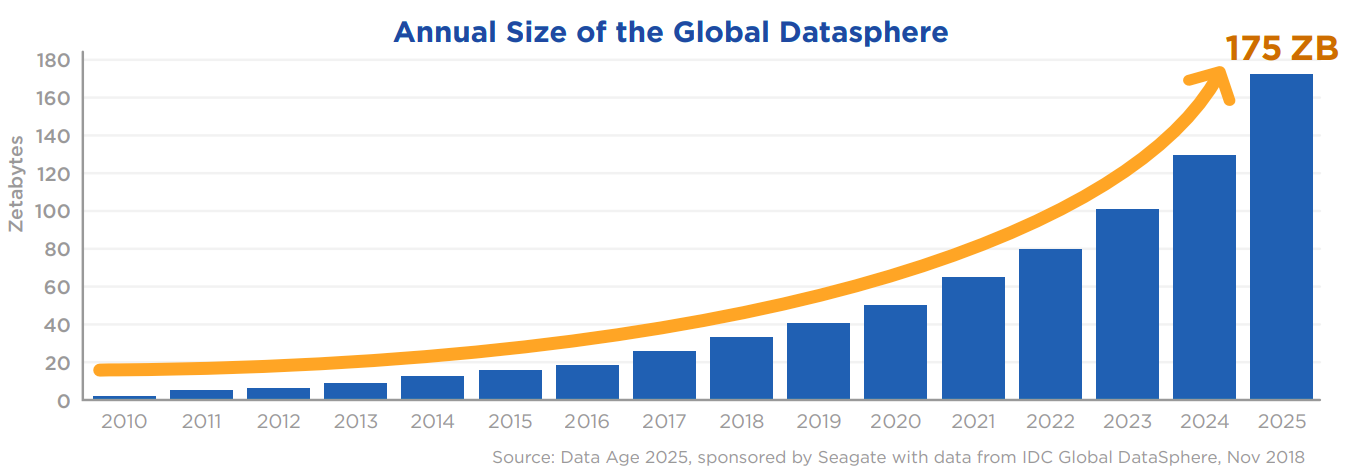
\includegraphics[width=1.0\textwidth]{Bilder/size_global_datasphere.png}
\caption{The Growth of the Global Datasphere \cite[p.6]{idc-seagate-data}}
\label{fig:growth_datasphere}
\end{figure}

% Maybe a source here?
Data has become an important factor in decision making and optimization in virtually every industry, especially in finances. \textbf{TODO: Wieso? Vllt sogar diese Section ueberarbeiten}
The financial market is dominated by data driven decisions, with emphasis on data processing, often in a (near) real-time fashion.
However, real-time data is becoming of importance in multiple sectors; the International Data Corporation estimates that real-time data will be 
responsible for a share of 30 percent of the total global datasphere by 2025, as shown in figure \ref{fig:growth_realtime_data}.
% Graph showing the growing share of real-time data as part of global datasphere
\begin{figure}[ht]
\centering
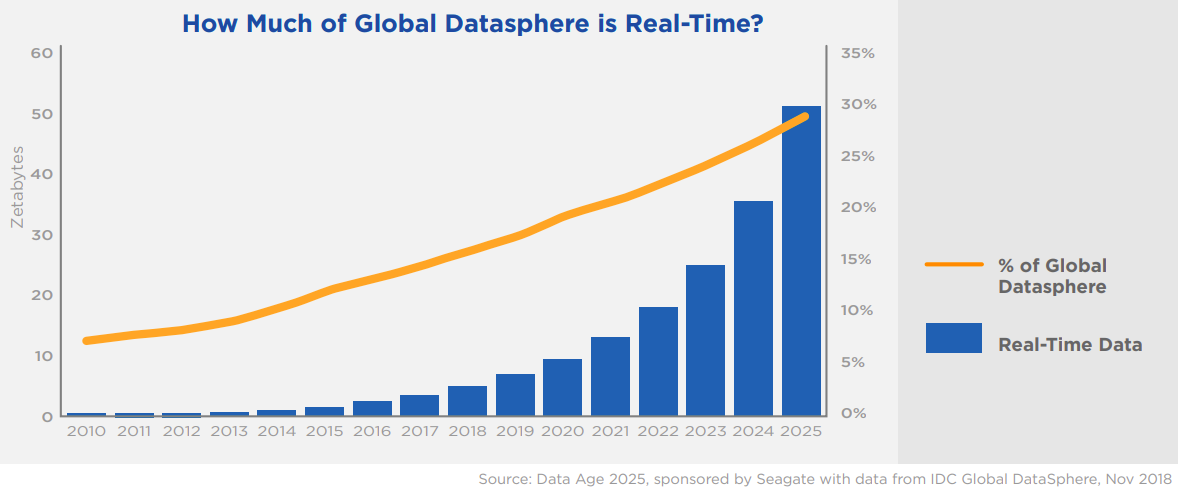
\includegraphics[width=1.0\textwidth]{Bilder/realtime_data.png}
\caption{The growth of real-time data as part of the Global Datasphere \cite[p.13]{idc-seagate-data}}
\label{fig:growth_realtime_data}
\end{figure}

A global study led by IBM in 2012 has shown that 71 percent of the firms in the financial market use information (including big data)
in order to achieve an advantage over their competitors, compared to 36 percent, which IBM has found in an earlier study conducted in 2010. \cite[p.1]{ibm-financial}

As it is no longer feasible to save all the data before then analyzing it (in batches), due to computational cost and lack of storage capacity, 
a new approach was designed in order to handle data in a (near) real-time fashion, stream processing systems (SPS). 
A stream processing system takes in a continuous stream of data and processes each element of said stream, and then puts out a stream of processed data.
These systems will further be explained in \ref{sub:sps} \nameref{sub:sps}.
\\
However the rate in which data is being streamed fluctuates, so one comes to the logical conclusion that SPSs should adapt to the velocity and volume of the stream.
Besides the stream, the computing environment might also fluctuate, e.g. a resource failing in a distributed computing environment, 
and as such the system has to adapt. There are many different techniques of adaptation such a system might utilize, 
which can impact both the stream as well as the SPS. We will elaborate on this in \ref{sub:sps} \nameref{sub:sps}.

In this thesis our goals are to define stream processing and to look at various adaptation techniques in stream processing. Furthermore we will clarify why
self-adaptivity is needed in stream processing and what current architectures, that enable self-adaptivity in stream processing, look like.
We will also discuss the impact of self-adaptivity on software engineering, especially in stream processing.


\section{Structure}
\label{sec:structure}
\textbf{\color{green}THIS IS FINAL}

In chapter \ref{cha:Introduction} we will introduce the topic, and explain the motivation and structure of the thesis.

In chapter \ref{cha:fundamentals} we will go over the fundamental concepts regarding the general topic of stream processing and adaptive systems.
\\
In section \ref{sec:stream-processing} stream processing will be explained by first clarifying data stream management systems and comparing them to database management systems 
in \ref{sub:dsms}, afterwards we will look into steam processing systems and understand how they work and the challenges they're facing.
\\
In \ref{sub:requirements} we will then discuss requirements as formulated by Stonebraker et al. and explore how they influence our decisions when designing system architectures.
\\
In section \ref{sec:self-adaptive} we will then introduce the concept of self-adaptive systems and their design, including the MAPE-loop in \ref{sub:mape}. 
Furthermore, we will discuss self-adaptivity's impact on software engineering.
\\
In chapter \ref{cha:approaches} we then discuss several architectural approaches in designing self-adaptive stream processing systems, starting with Dhalion in \ref{sec:dhalion}, 
followed by a decentralized approach by Cardellini et al. in \ref{sec:hierarchical}.
Each subsection of this chapter will contain a thorough description of the approach's architecture followed by a discussion, 
in which they will also be compared to their reference architecture, the MAPE-loop.
\\
Chapter \ref{cha:summary} will then provide a summary of our findings and conclude the thesis.